% Version 2019-01-08
% update – 161114 by Ken Arroyo Ohori: made spacing closer to Word template throughout, put proper quotes everywhere, removed spacing that could cause labels to be wrong, added non-breaking and inter-sentence spacing where applicable, removed explicit newlines
% update – 010819 by Dennis Wittich: made spacing and font size closer to Word template, updated references and refernces style
% update – 042319 by Dennis Wittich: font size of captions set to 'small', first author names are shortened, hyphenation fixed

\documentclass{isprs} % isprs class modified 23-04-2019 (Dennis Wittich)
\usepackage{subfigure}
\usepackage{setspace}
\usepackage{geometry} % added 27-02-2014 Markus Englich
\usepackage{epstopdf}
\usepackage[labelsep=period]{caption}  % added 14-04-2016 Markus Englich - Recommendation by Sebastian Brocks
\usepackage[british]{babel} 

\geometry{a4paper, top=25mm, left=20mm, right=20mm, bottom=25mm, headsep=10mm, footskip=12mm} % added 27-02-2014 Markus Englich
%\usepackage{enumitem}

%\usepackage{isprs}
%\usepackage[perpage,para,symbol*]{footmisc}

%\renewcommand*{\thefootnote}{\fnsymbol{footnote}}
\captionsetup{justification=centering,font=normal} % thanks to Niclas Borlin 05-05-2016
\captionsetup[figure]{font=small} % added 23-04-2019 Dennis Wittich
\captionsetup[table]{font=small} % added 23-04-2019 Dennis Wittich

\begin{document}

\title{SMODERP2D SOIL EROSION MODEL ENTERING AN OPEN SOURCE ERA WITH
  GPU-BASED PARALLELIZATION}

% KAO: Remove extra spacing
\author{
 M. Landa\textsuperscript{1}, J. Jeřábek\textsuperscript{2}, O. Pešek\textsuperscript{1}, P. Kavka\textsuperscript{2}}

% KAO: Remove extra newline
\address{
  \textsuperscript{1 }Dept.\ of Geomatics, Faculty of Civil Engineering, Czech Technical University in Prague,\\ Czech Republic - (martin.landa, ondrej.pesek)@fsv.cvut.cz\\
  \textsuperscript{2 }Dept.\ of Landscape Water Conservation, Faculty of Civil Engineering, Czech Technical University in Prague,\\ Czech Republic - (jakub.jerabek, petr.kavka)@fsv.cvut.cz\\
}

% If the corresponding author is NOT the final author, always add a % space before the subsequent comma, i.e.
% first author name\textsuperscript{a,}\thanks{Corresponding author} , % second author name \textsuperscript{b}, etc.
% thanks to Niclas Borlin 05-05-2016


\commission{VI, }{VI} %This field is optional.
\workinggroup{VI/4} %This field is optional.
\icwg{}   %This field is optional.

% KAO: Use times symbol
\abstract{ SMODERP2D is a runoff-soil erosion physically-based
  distributed episodic model used for calculation and prediction
  processes at agricultural areas and small watersheds. The core of
  the model is a raster based cell-by-cell mass balance calculation
  which includes the key hydrological processes, such as effective
  precipitation, surface runoff and stream network routing. Effective
  precipitation, the forcing of the runoff and erosion processes, is
  reduced by surface retention and infiltration. Surface runoff
  consists of two components: slower sheet and concentrated rapid rill
  flow. Stream network routing is performed line-by-line in user
  predefined polyline layer.

  SMODERP is a long-term running project driven by the Department of
  Landscape Water Conservation at the Czech Technical University in
  Prague. At the beginning SMODERP has been developed as a surface
  runoff simulated by profile model (1D). Later the model has been
  redesigned using spatially distributed method. This version is named
  SMODERP2D. Ongoing development is focused on obtaining parameters of
  the hydrological models, incorporating new infiltration and flow
  routing routines, and conceptualization of a rill flow and rill
  development. The model belongs to a family of so called GIS-based
  hydrological models utilizing capabilities of GIS software for
  geodata processing. Importantly, the SMODERP2D project is currently
  entering the open source world. Originally the model could be run
  only in proprietary Esri ArcGIS platform. A new version of the model
  presented by this contribution adds support for two key open source
  GIS platforms, GRASS GIS and QGIS. A newly developed GRASS module
  and QGIS plugin significantly increases accessibility of the
  SMODERP2D model for research purposes and also for engineering
  practice.

  Middle scale distributed hydrological models often encounter with a
  high computation costs and long model runtime. Long runtime is
  caused by high resolution input data which is easily available
  nowadays. The project also includes an experimental version of the
  SMODERP2D model enabling the parallelization of computations. This
  parallelization is done using TensorFlow, and its goal is to
  decrease the time needed for its run. It is supported by both CPU
  and GPU. Parallelization of computations is an important step
  towards providing SMODERP2D web processing services in order to
  allow quick and easy integration to highly specialized platforms
  such as Atlas Ltd.  }

\keywords{Hydrology, Soil Erosion Models, GIS, Open Source, Parallel computing}

\maketitle

%\saythanks % added 28-02-2014 Markus Englich

\section{INTRODUCTION}\label{INTRODUCTION}
 
% KAO: Sloppy spacing ensures non-overfull lines. Can be removed if this is not an issue.
\sloppy

Erosion / hydrological models (EH) are being used for various research or engineering purposes. Results of such a model may be used as an input information for a planning or designing soil conservation measures. Volumes of runoff water and transported soil amounts or time series of runoff water may be calculated so the dimension of the protection measure is sufficient for a given flood or soil transport event. Another example of a practical application of EH models may be studies of land-use change or build up areas development effect on the soil and water transport at an area of interest. Great use of EH models is also in extreme event forecasting. For research purposes EH models are being used to proof a new theory or to test a hypothesis of mechanisms controlling the runoff and erosion.

Empirical erosion models are often based on Universal Soil Loss Equation (USLE), (Wischmaier, 1978, Renard, 1997) and empirical hydrological models on Curve number method (CN) (USDA, 1986), concepts more than 30 years old. Using empirical approaches may introduce limitations in designing the protection measures. Physically based models are being developed to overcome the empirical models limitations. 

Surface processes are spatially distributed, which is the reason why GIS is often depling in the modeling process taking advantage of ready to use GIS features EH models have similar structure (although each model is specific in terms in solved processes, its purpose or coding strategy). The forcing is precipitation which is often introduced in the model in spatially distributed manner. Majority of models contain an infiltration routine which parameters may be spatially distributed since grass land or parking lot may be presented in single hydrological model and have vastly distinct infiltration characteristic. Infiltrated water is transported to the soil with different transport properties. Ponging water creates overland flow which leads to a soil transport and may case sever soil and nutrition losses. In the modeled system may be presented linear (water courses, streets, ditches) or points (typically a water pump) features which affect the water flow and soil transport routines as well. 


The EH model may encounter with some run-time issues which rise from model spatial and temporal discretization. It was noted in Molnar & Julien, (2000) that grid cell size is interchangeable in terms of spatial discretization if the model parameters were calibrated on the model with the same grid size. Data availability and larger computation resources lead more often to the use of finer spatial resolution. This may, in some cases, cause problems with time discretization which is commonly controlled with Courant–Friedrichs–Lewy (CFL) criterion. CFL criterion force the time step to be lower if velocity of flow process increases or the spatial discretization become finer. Maximum allowed value of CFL criterion theoretically equals one. For shallow surface processes (processes which take place in the used model) CFL should be even smaller than one, as it was noted in Zhang & Cundy (1989) or Esteves et al. (2000). The need for smaller time step is caused mainly by discrepancy between solution height (surface water) and cell size and surface roughness coefficient or sharp surface slope changes between adjacent cells. 

In case of EH models the commonly computed processes are sheet (water covers the earth's surface evenly) and rill flow (water detaches the soil material and concentrates its flow in the created rill). Although the concentrated rill flow is particularly fast (causing  the time step size constrain) it is usually not spatially extensive over the watershed. The rill flow usually occurs at concentrated flow paths. The computation may end up in a situation where a small portion of the computation domain force shorter time step (due to rill flow)  whereas the rest of the area allows a large one. In that case only a small part of the computed watershed causes the long model run-time. 


Nevýhoda -  Výpočet je numericky náročný, kuli CFL
Procesy jsou rychlé jen v některých buňkách, ostatní části “čekají”
Jedním z přístupů je využití rozbusnosti výpočetní techniky. 
TO je umožněno paralezlazcí výpočtu (CPU/GPU). Princip pravidelné mřížky -  nejsnazší, princip      subpovodí     

Testování jak využít paralelizaci je testováno na modelu SMODERP..


\section{MATERIAL AND METHODS}\label{sec:mat_met}

\subsection{SMODERP2D model}
The SMODERP2D model has a simple structure based on mass balance equation:
\begin{equation}\label{equ:mass_bal}
    \frac{Storage}{\Delta t} = \nonumber  
    Inflow - Outflow
\end{equation}
In equation~(\ref{equ:mass_bal}) the Storage is represented by
surface water level which $h$ [$L$] which changes each proceeding time
during the computation.

The $Inflow$ and $Outflow$ terms on the right-hand side of
equation~(\ref{equ:mass_bal}) consist of several components and are
defined for each $i_th$ cell in the computation domain:
\begin{equation}\label{equ:inflow}
    Inflow_i = es_{i} + \sum_j^n q_{j}
\end{equation}
\begin{equation}\label{equ:outflow}
    Outflow_i = inf_{i} - q_{i} - ret_i
\end{equation}
\begin{tabbing} 
where \hspace{0.6cm} \= $es$ = effective precipitation\\
\> $q$ = inflow to resp. outflow from a given raster cell\\
\> $inf$ = infiltration\\
\> $ret$ = surface retention for a given raster cell
\end{tabbing}
The sum $\sum_j^n$ indicates that there can be more that one cell
flowing in cell i. The flow direction and therefore the sum $\sum_j^n$
is controlled be $D8$ flow direction algorithm~\cite{ocallaghan1984}.  Effective
precipitation $es$ is potential precipitation reduced by
interception of the rainfall water on the vegetation.

The model is forced to satisfy the Courant–Friedrichs–Lewy (CFL)
criteria~\cite{courant1928}:
\begin{equation}\label{equ:CFL}
    CFL = \frac{q\textrm{d}t}{\textrm{d}x} < 1.0
\end{equation}
\begin{tabbing} 
where \hspace{0.6cm} \= $\textrm{d}t$ = time step\\
\> $\textrm{d}x$ = grid cell size
\end{tabbing}
If the flow $q$ in the cell highs the model is forced to decrease the
time step in order to satisfy the CFL criteria, since grid cell size
is fixed.

The flow $q$ in equation~(\ref{equ:inflow}) and~(\ref{equ:outflow})
has two components. Slower and spatially extensive sheet flow
$q_{sh}$:
\begin{equation}\label{equ:sheetflow}
    q_{sh} = XI^Yh^b
\end{equation}
\begin{tabbing} 
where \hspace{0.6cm} \= $X,Y,b$ = empirical parameters\\
\> $I$ = surface slope
\end{tabbing}
and faster concentrated rill flow $q_{rl}$ calculated by Mannings formula:
\begin{equation}\label{equ:rillflow}
    q_{rl} = A\frac{1}{n} R^{2/3} I^{1/2}
\end{equation}
\begin{tabbing} 
where \hspace{0.6cm} \= $A$ = cross-section area\\
\> $n$ = roughness in the rill\\
\> $R$ = hydraulic radii
\end{tabbing}
The resulting flow is a sum of sheet and rill flow:
\begin{equation}\label{equ:flow}
    q = q_{rl} + q_{rl}
\end{equation}

Infiltration is solved with Phillip's infiltration equation \cite{philip1957theory}:
\begin{equation}\label{eq:Phillips}
    inf = 1/2St^{-1/2} + Ks
\end{equation}
\begin{tabbing} 
where \hspace{0.6cm} \= $S$ = sorptivity\\
\> $K_s$ = hydraulic conductivity
\end{tabbing}

The reason why the parallelization is considered is the flow
in~(\ref{equ:flow}). Parameters of
relations~(\ref{equ:sheetflow})~(\ref{equ:rillflow}) and
(\ref{eq:Phillips}) may be spatially distributed. And the data are
handled by Esri ArcGIS, QGIS and GRASS GIS providers, see
\ref{ref:open_source_providers}.


\subsection{SMODERP2D entering an open source world}\label{ref:open_source_providers}

SMODERP2D is a project with a long history. Over the years its
development has been driven by the Department of Landscape Water
Conservation at the Czech Technical University in Prague. In 2018
SMODERP2D developers started working on a new generation of the model
in order to solve or at least to improve various critical issues of
the project. This includes most importantly a computation stability
and performance, better interoperability, and lack of
documentation. Recently SMODERP2D source code has been published on
GitHub \cite{smoderp2d-github-2019} under GNU GPL licence in order to
attract a wider audience, new developers and users.

The model is implemented in Python programming language using the
object-oriented paradigm. The original source code has been designed
with a low level of a scalability, limited readability and
interoperability. Part of the computation phase responsible for a data
preparation was restricted to a single platform only, Esri ArcGIS. In
2018 the original source code has been completely refactorized. Python
classes defining computational steps were re-organized in a
hierarchical manner. Major design-related changes have been done in
Python classes responsible for data handling and preparation using GIS
software tools. Data preparation workflow is handled by a
newly-defined base, partly abstract Python class ({\tt BaseProvider},
fig.~\ref{fig:uml_diagram}). Functionality depending on used GIS
package has been separated into new classes. This step was crucial in
order to make data preparation workflow GIS package independent. The
only supported platform, Esri ArcGIS, has been separated from a base
workflow. Based on that, a new concept of so-called “GIS providers”
has been introduced, see fig. \ref{fig:uml_diagram}. The key point is
the separation of GIS functionality related code from generic workflow
defined by the base provider. The base provider depends only on
standard builtin Python libraries. Array-like computation is performed
by a well-known Numpy library. Using GIS provider prototypes, the
SMODERP2D project can be easily extended to support another GIS
packages responsible for the data preparation phase. 

\begin{figure}[ht!]
  \begin{center}
    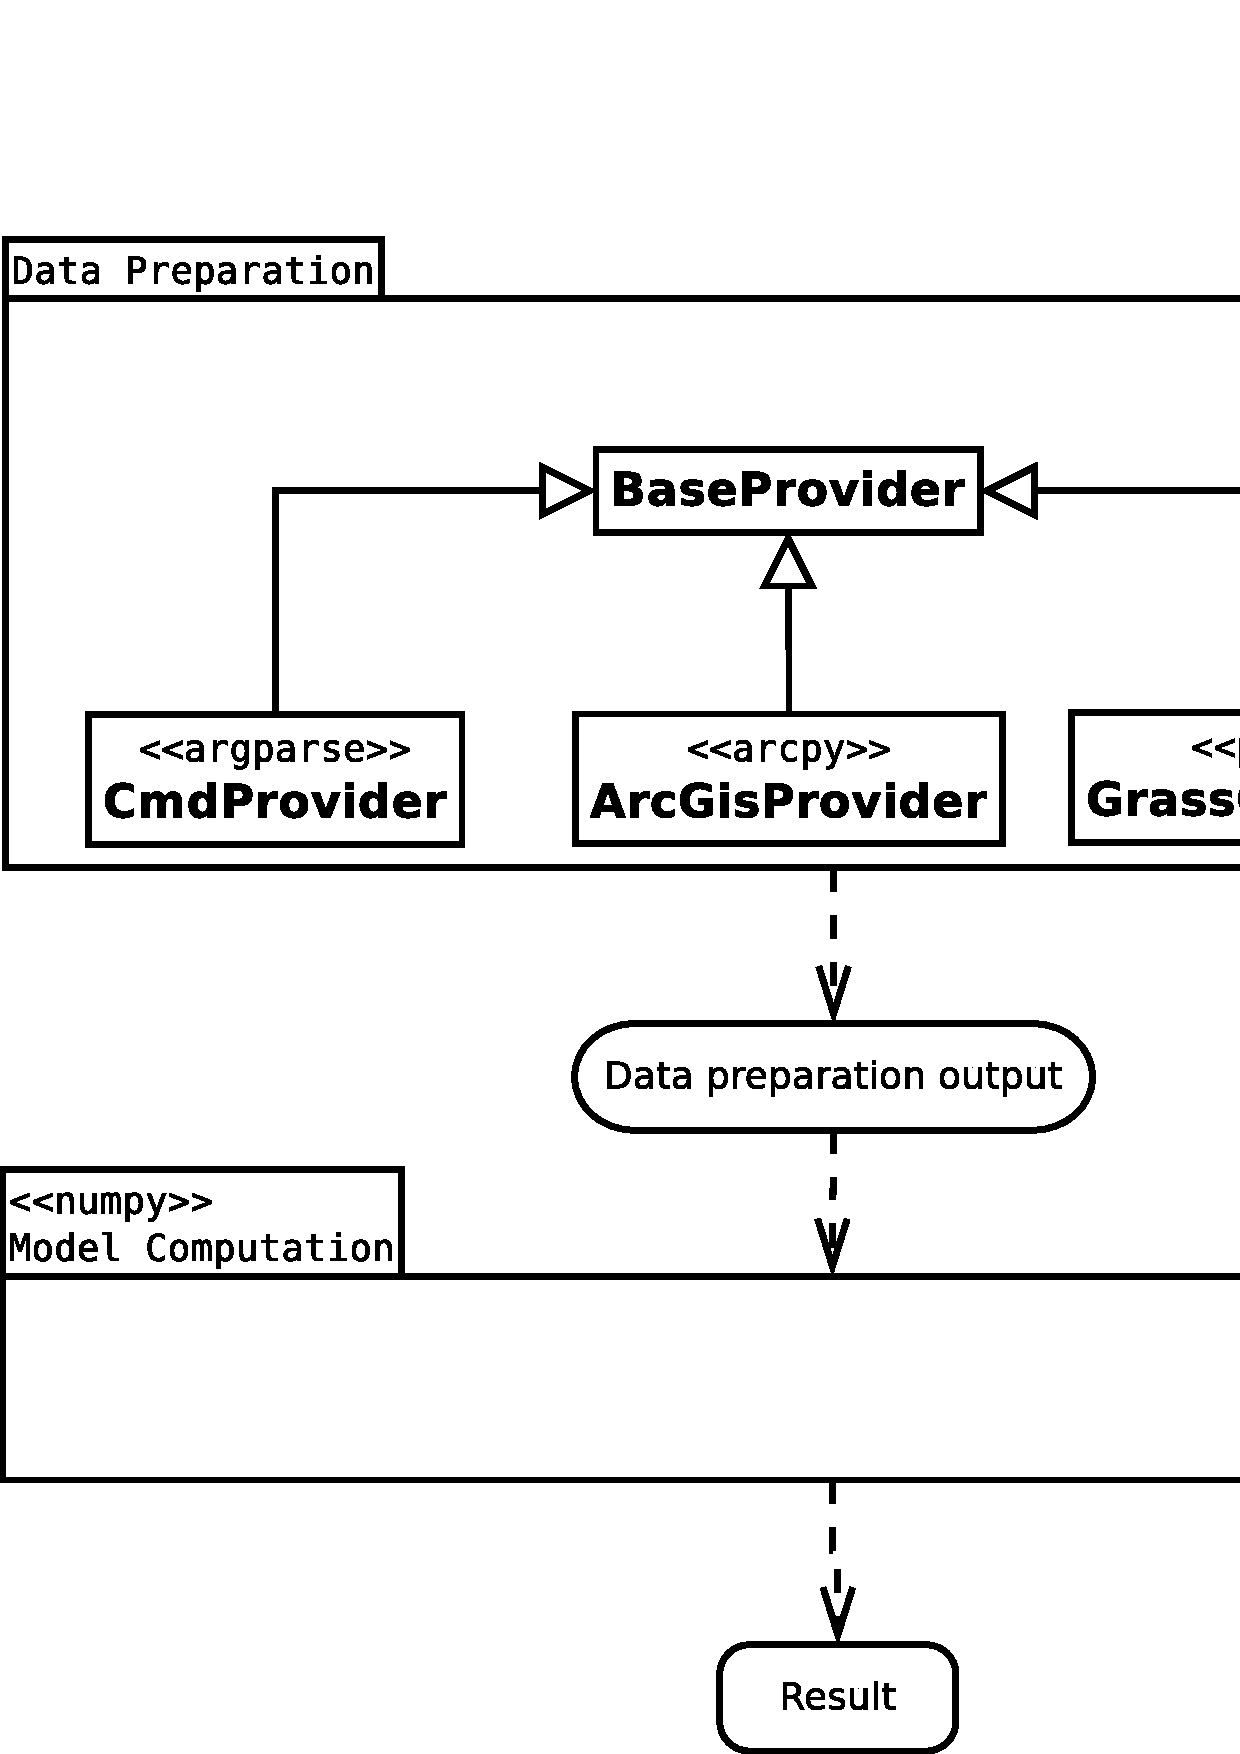
\includegraphics[width=1.0\columnwidth]{figures/uml_diagram.pdf}
    \caption{Concept of GIS providers}
    \label{fig:uml_diagram}
  \end{center}
\end{figure}

Currently the SMODERP2D project comes with three different GIS
providers. Support for Esri ArcGIS platform is implemented by {\tt
  ArcGISProvider}, GRASS GIS is handled by {\tt GrassGisProvider}, see
\ref{sec:grass_provider}. The {\tt CmdProvider} is triggered only when
model computation is run from a command-line. In this case it is
assumed that data preparation phase has been already performed by one
of supported GIS platforms.

Example of running computation from a command-line. Option {\it
  --typecomp roff} specifies that only model computation without data
preparation phase is triggered. It means that data has been already
prepared and stored in a pickle file distributed by {\it test.ini}
configuration file.

\begin{verbatim}
./bin/start-smoderp2d.py --typecomp roff \
 --indata tests/test.ini
\end{verbatim}

\subsubsection{GRASS GIS integration}\label{sec:grass_provider}
Importantly, the new SMODERP2D version extends supported GIS providers
by a GRASS-based provider. Introducing an open source GIS platform to
SMODERP2D workflow is crucial from the perspective of
interoperability. SMODERP2D users can choose between a proprietary
Esri ArcGIS platform and an open source GRASS GIS
\cite{neteler2012grass}. The GRASS GIS provider is designed similarly
to ArcGIS provider. From a Python perspective, there is only one
difference, GIS functions are accessed by PyGRASS package
\cite{ijgi2010201}. Nevertheless, an integration of GRASS tools in the
SMODERP2D project required a few improvements in GRASS GIS
itself. That was possible since GRASS GIS is an open source project
available under GNU GPL licence. These improvements have been
integrated into main GRASS GIS distribution and will be part of
upcomming GRASS GIS version 7.8.  GRASS v.to.points module
\cite{v-to-points-2019} has been extended to extract from lines start
or end nodes only. This functionality is used to determine the slope
of a polyline stream feature to ensure that its direction will always
be downslope (see fig. \ref{fig:stream_next_edge}). Another
improvement has been done in v.to.db GRASS module
\cite{v-to-db-2019}. This tool allows uploading geometry-related
information into the attribute table. Newly added option {\it
  next\_edge} allows adding information about next left and right
edge. This functionality is important for SMODERP2D in order to
determine stream network connectivity, see
fig. \ref{fig:stream_next_edge}.

\begin{figure}[ht!]
  \begin{center}
    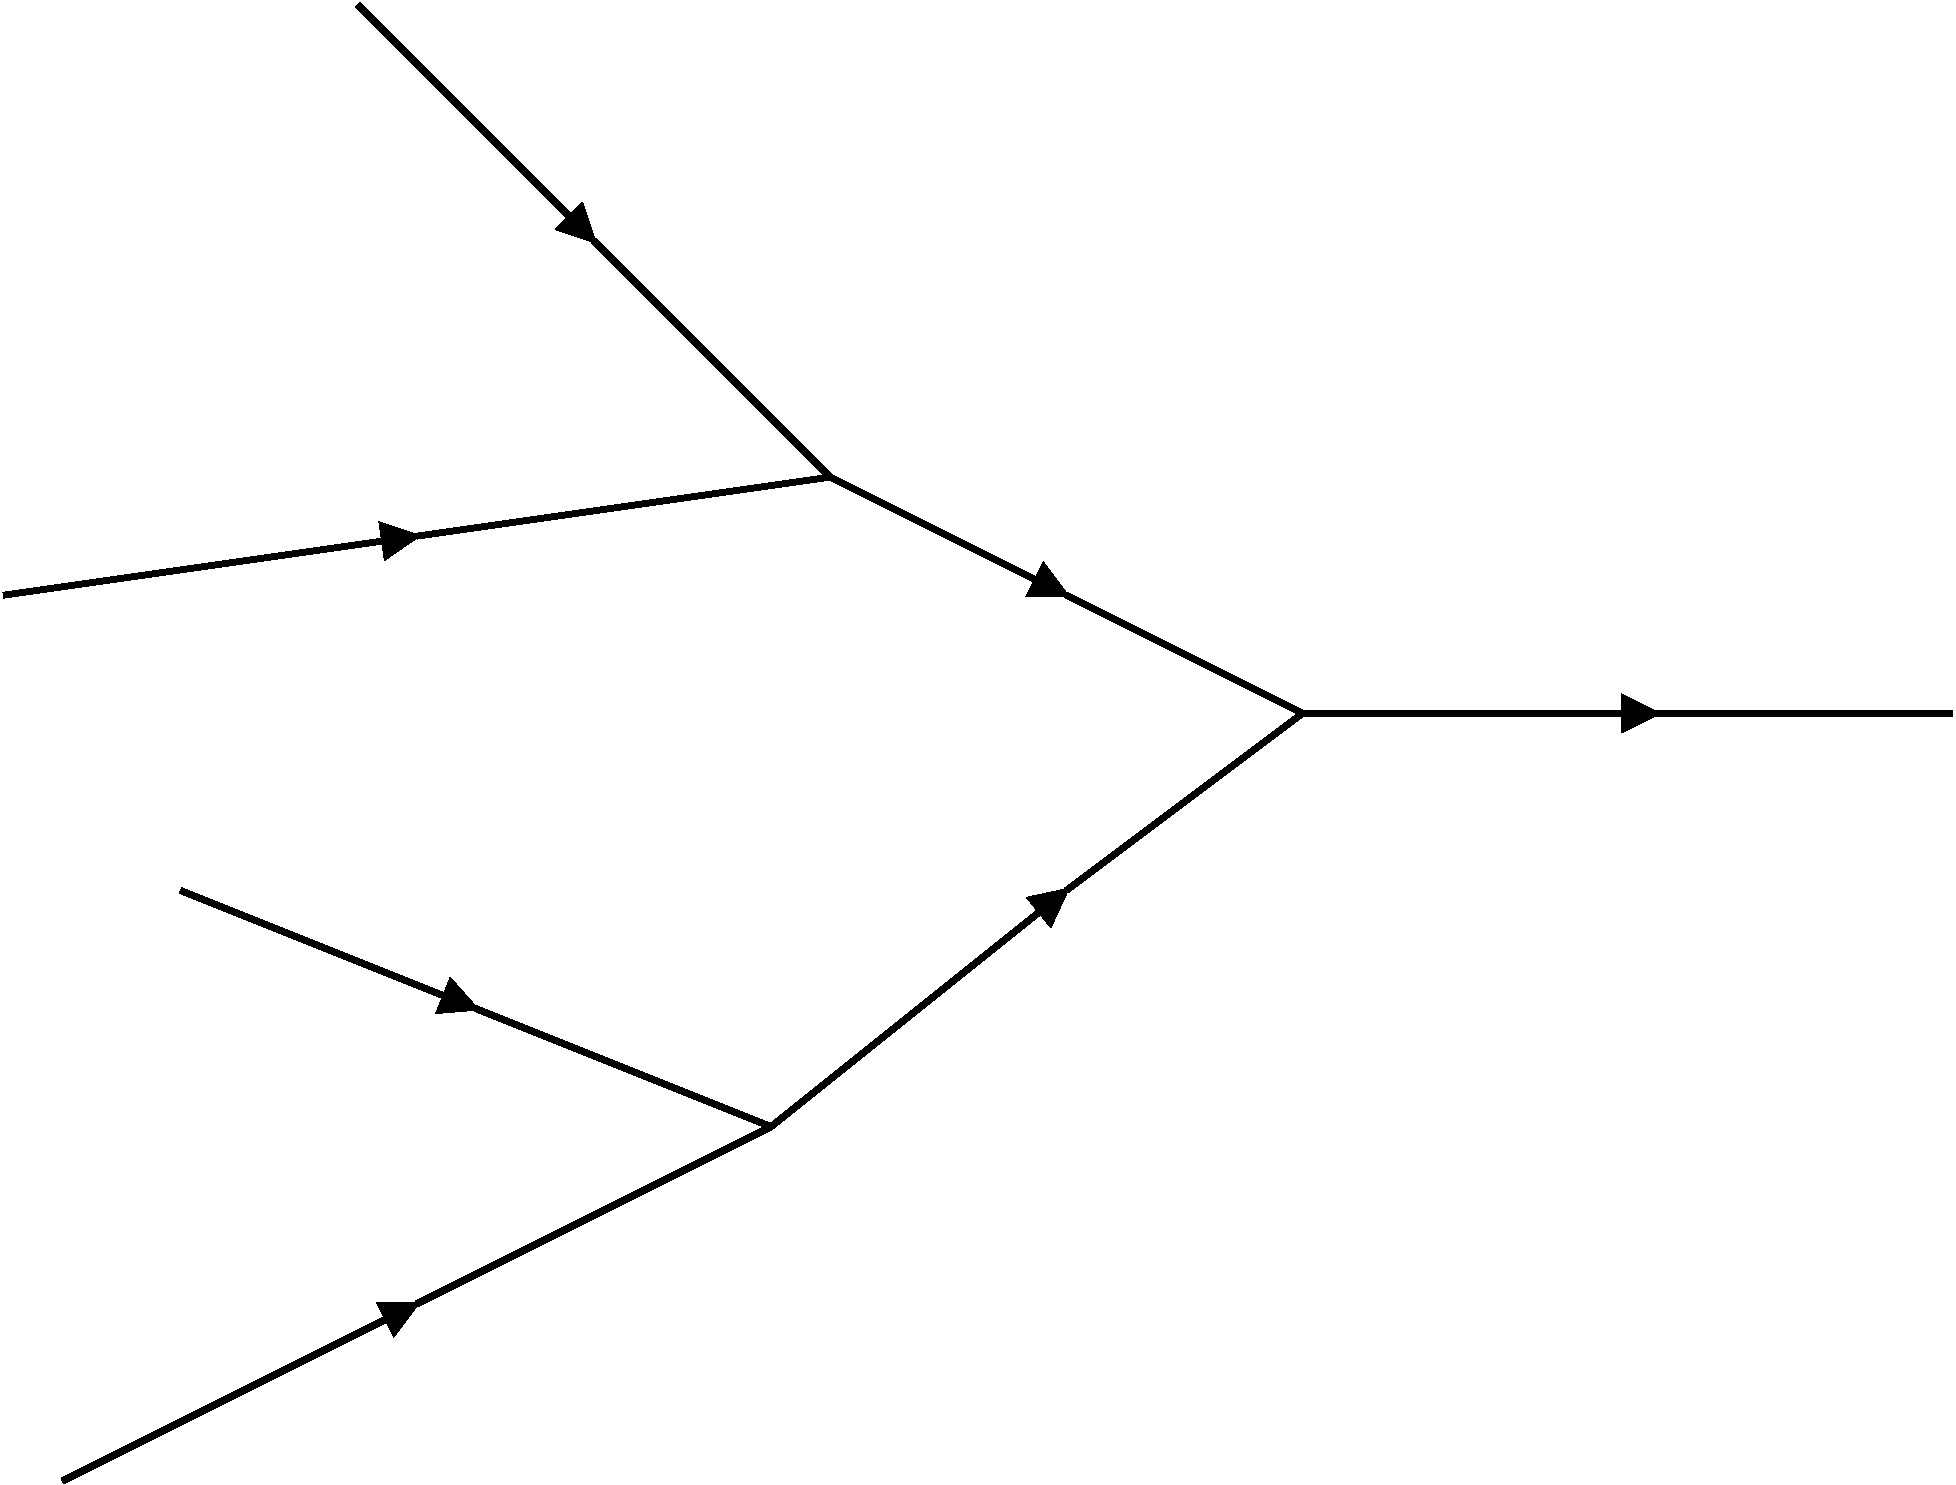
\includegraphics[width=0.6\columnwidth]{figures/stream_next_edge}
    \caption{Stream segmentation procedure network connectivity}
    \label{fig:stream_next_edge}
  \end{center}
\end{figure}

On the top of GRASS GIS provider a specialized GRASS {\em r.smoderp2d}
module has been designed. This tool allows an user running SMODERP2D
model computation directly from GRASS GIS working environment, see
fig. \ref{fig:r.smoderp2d}. The module can be easily installed in
GRASS GIS similarly to other extensions (so-called addons modules) by
{\em g.extension} command. By default, the {\em r.smoderp2d} module
performs data preparation phase followed by a model computation. Data
preparation only can be performed by {\em -d} flag. In this case, the
module creates a binary pickle file which can be later used for a
subsequent model computation. Note that ArcGIS Toolbox also allows
creating a pickle file for later usage. Importantly, such pickle files
are platform independent.

{\em r.smoderp2d} command-line usage example:
\begin{verbatim}
r.smoderp2d elevation=w001001 soil=soil_map \
 soil_type=Novak vegetation=soil_map \
 vegetation_type=veg rainfall_file=rainfall.txt \
 points=points2 table_soil_vegetation=tab_sv \
 table_soil_vegetation_code=soilveg \
 table_stream_shape=tab_stream_shape \
 table_stream_shape_code=smoderp stream=stream 
\end{verbatim}

\begin{figure}[ht!]
  \begin{center}
    \includegraphics[width=1.0\columnwidth]{figures/smoderp2d_grass.png}
    \caption{Running r.smoderp2d module from GRASS graphical user interface}
    \label{fig:r.smoderp2d}
  \end{center}
\end{figure}

\subsubsection{QGIS plugin}
Recently the SMODERP2D model has been integrated also into QGIS
environment. QGIS\footnote{https://www.qgis.org} is a widely used open
source GIS platform which can be easily extended by user-defined
plugins. A SMODERP2D QGIS plugin allows performing both data
preparatation and model computation phases in QGIS native environment,
see fig.~\ref{fig:smoderp2_qgis}. Data preparation part is ensured by
GRASS GIS provider as described in \ref{sec:grass_provider}. Note that
QGIS installation normally comes with GRASS GIS included. It means
that GRASS dependency is solved by QGIS installation
itself. Experimental code of the plugin compatible with the current
long term release QGIS version 3.4 is available from project GitHub
repository \cite{smoderp2d-github-2019}.

\begin{figure}[ht!]
  \begin{center}
    \includegraphics[width=1.0\columnwidth]{figures/smoderp2d_qgis.png}
    \caption{SMODERP2D model implemented as QGIS plugin}
    \label{fig:smoderp2_qgis}
  \end{center}
\end{figure}

\subsubsection{Python3 support}
SMODERP2D project also comes with Python 3 support, but still
supporting Python 2. Note that Python versions 2 and 3 are not
backward compatible.  Python~3 support is important from various
perspectives. Python 2 is slowly reaching end of
life\footnote{https://legacy.python.org/dev/peps/pep-0373/}, but still
it’s used by many GIS platforms such Esri ArcGIS 10.x. Newly supported
GIS platforms by the SMODERP2D project as Esri ArcGIS Pro, (upcoming)
GRASS GIS 7.8 and QGIS 3.x are Python 3 based. On the other hand it’s
still meaningful to support both Python versions, Python 2 mainly
because of Esri ArcGIS 10.x platform.

\begin{figure}[ht!]
  \begin{center}
    \includegraphics[width=1.0\columnwidth]{figures/smoderp2d_arcgis.png}
    \caption{SMODERP2D model available as ArcToolbox for Esri ArcGIS
      10.x and Pro platforms}
    \label{fig:smoderp2d_arcgis}
  \end{center}
\end{figure}


\subsection{Parallel computing experiments}

Because one of the most crucial points of SMODERP2D computations is
the speed, an experimental branch allowing (both CPU and GPU-based)
parallelised computations has been developed.

The main step was to rewrite all loop-based computations into
matrix-based mathematical operations. To keep matrices as so-called
tensors and to perform all the operations, an open source  TensorFlow Python
library \cite{tensorflow2015-whitepaper} developed by Google Brain
Team\footnote{https://ai.google/research/teams/brain/} was used. Even though
TensorFlow is most widely used for machine learning
and its performance on basic mathematical operations is not always better
than the one of NumPy (a quick comparison with NumPy and Numba can be
seen in \cite{tf-np}), it had been preferred for its easy switch
between CPU and GPU-based core (it depends only on the version of
TensorFlow the user has installed, no needs for changes in code) and
therefore support also for users without an access to machines with
GPU. Another advantage of TensorFlow is its usage of so-called
graphs. A graph is a representation of all operations in
dataflow/workflow and its individual operations are automatically sent
to multiple cores in a CPU or multiple threads in a GPU. These nodes
are run independently in parallel.

To support further development of TensorFlow and exploit its bleeding
edge functionalities, TensorFlow 2.0, which is published currently
just as an alpha version, was used in the SMODERP2D experimental
branch. Because TensorFlow 2.0 is still not suitable with all the
Python acrobatic tricks, NumPy was used for matrix operations in
places where TensorFlow could not (on places where loops were still
needed; looping through a NumPy array is incomparably faster than
through a Tensor).

This experimental SMODERP2D branch is still under development;
however, the alpha-version is ready to be used. Table \ref{tab:GPU_results}
presents the results of different tests made on this version
(comparing parallelized GPU computation, parallelized CPU computation and a single CPU one).

\begin{table}[h]
  \centering
  \caption{Results of parallelization tests}
  \makegapedcells
  \begin{tabular}{|l|p{2.2cm}|c|c|}\hline
    RAM & Processing unit & Data 62 KB & Data 197 MB\\
     & & [s] & [s]\\\hline
    \multirow{3}{*}{15 GB} & GPU1 & 4.0 & 7 560\\
    & CPU1 & 0.2 & 12 809\\
    & CPU2 & 2.1 & 7 249\\\hline
    \multirow{3}{*}{251 GB} & GPU2 & 2.5 & 6 611\\
    & CPU3 & 0.2 & 10 637\\
    & CPU4 & 1.5 & 8 631\\\hline
  \end{tabular}
  \label{tab:GPU_results}
  \caption{Used processing units}
  \begin{tabular}{|l|p{1.9cm}|c|c|}\hline
    ID & Model & Clock speed & Memory\\\hline
    GPU1 & GeForce GTX 1060 3GB & 33 MHz & 3 016 MiB \\\hline
    GPU2 & $4\times$ GeForce GTX 1080 Ti & 33 MHz & 11 178 MiB \\\hline
    CPU1 & AMD Ryzen 7 1700 Eight Core Processor & 1 373 MHz & 512 KB \\\hline
    CPU2 & $16\times$ AMD Ryzen 7 1700 Eight Core Processor & 1 373 MHz & 512 KB \\\hline
    CPU3 & Intel Xeon CPU E5-2630 v4 @ 2.20 GHz & 2 423 MHz & 25 600 KB \\\hline
    CPU4 & $40\times$ Intel Xeon CPU E5-2630 v4 @ 2.20 GHz & 2 423 MHz & 25 600 KB \\\hline
  \end{tabular}
\end{table}

As can be seen in the table, the usage of GPUs is not always
the~right way even when compared with CPUs, both single and parallelized ones.
The bottleneck of TensorFlow is its graph initialization; this step is very
time-consuming and therefore can last many times longer than the computation
itself for extremely small data. Another bottleneck is the memory shift between RAM and GPU virtual memory which concludes into slower processes for weaker GPUs (compared with parallelized computations being run on CPUs). Generally, for data of common size
was the process with parallelized computations faster (reaching around 60 per cent of the total
computation time on different architectures). Interesting moment is slower run of much stronger $CPU4$ when compared with weaker $CPU2$; this behaviour has to be examined deeper. 

\subsubsection{Further ideas for a sub-basins based parallel computing}
Besides the GPU-based parallelization (with TensorFlow \cite{tensorflow2015-whitepaper} or
NVIDIA Cuda technology~\cite{Kalyanapu2011,Le2015}) the
pure CPU-parallelization may also bring a good improvement in the computation
time reduction. The computation domain is separated into sub-domains
based on a certain algorithm where each sub-domain computation is loaded to a single
CPU core.  It is beneficial to incorporate the
hydrological behaviour in the parallelization
strategy if the domain is a hydrological basin. 
In~\cite{Vivoni2011} the basin was separated in sub-basins
based on stream network. The sub-basins communicated with each other through so-called
ghost cell. The strategy aimed to generate as few ghost cells as
possible; to reduce the communication between the CPU cores. 

The parallelization strategy outlined in the manuscript is based on
the hydrological reality and it is shown in a simplified setup in Figure~\ref{fig:cpu-parallel}. In this example, the Nu\v{c}ice experimental 
was chosen to present the parallelization strategy. At this 0.5 km$^2$ large 
basin a long-term monitoring of erosion and runoff processes is being conducted 
by the Dept.\ of Landscape Water Conservation. 

The strategy main goal is the reduction of
the communication between CPU-cores during the computation as much as
possible. The whole basin is divided into several sub-basins based on
the digital elevation model and user-defined sub-basin size. 
Outlet\footnote{the location in the basin where all water from the basin flows} 
of each sub-basin is depicted with
red dots in Figure~\ref{fig:cpu-parallel}. After the sub-basins
are defined, an order in which each sub-basin will be computed is defined as
follows. Sub-basins which are hydrologically the farthest from the
basin outlet (depicted by the triangle in Figure~\ref{fig:cpu-parallel}) 
and therefore have no inflow flow upslope area are
calculated at first. Those sub-basins have the rainfall stored in
hyetographs as the only input. In the simplified setup shown in
Figure~\ref{fig:cpu-parallel}, the sub-basins 1, 2, 3, and 6 are
calculated at first in parallel. The calculated hydrographs of the
sub-basins 1, 2, 3, and 6 are stored in the memory for the later use. 
Sub-basins which
have an inflow from sub-basins 1, 2, 3, and 6 are calculated next. It
this case it is the only the sub-basin 4. The water input in
the sub-basin 4 are now hyetograph and also hydrographs of
sub-basins 1 and 3. In the same manned are
calculated all sub-basins towards in the main basin outlet (red triangle in Figure~\ref{fig:cpu-parallel}) 
where its hydrograph is the desired outcome.

This approach may encounter several limitations. The main one 
originates from the basin geometry. In case of a narrow  basin a situation 
where each sub-basin has a single upslope and downslope sub-basin may occur.
In this case, the sub-basins will be computed in sequence, which
loses the advantage of multi-core working station. If this situation happens
the user will be forced to create very small sub-basins in order to be able 
to perform the outlined CPU-parallelization. The possibilities of CPU-parallelization
described in this section will be the subject of further research.


\begin{figure}[ht!]
  \begin{center}
    \includegraphics[width=1.0\columnwidth]{figures/smoderp-cpu-parallel.png}
    \caption{Simple example of possible CPU-parallelization strategy for the experimental catchment Nučice}
    \label{fig:cpu-parallel}
  \end{center}
\end{figure}






\section{CONCLUSION}

This manuscript presents SMODERP2D project and recently triggered 
development. Complete SMODERP2D source code is available on GitHub 
\cite{xxx} under GNU GPL licence. SMODERP2D computational tools have 
been successfully integrated into Esri ArcGIS, GRASS GIS and QGIS desktop GIS platforms. On top of that, the concept of so-called GIS providers allows publishing the SMODERP2D model as web processing service. Establishing experimental SMODERP2D 
OGC Web Processing Service is planned for 2019. Ongoing development 
is mainly focused on computational routines and parallel computations experiments. All the tools are currently distributed as experimental and are available for testing and user feedback.
The~official stable release of SMODERP2D model is planned in 2020. This 
includes also user documentation which is currently under development. 
In the 
case of SMODERP2D model, the run-time is an issue, especially 
if multiple mid-scale hydrological basins in fine spatial 
resolution grid computation needs to be undertaken. The code parallelization
is a common practice in cases where 
the reduction of run-time is convenient or even necessary, therefore
the existence of the TensorFlow-based branch; and although this branch is still
under development, the reduction of the computation costs is already reaching up to 40 per
cent depending on the data and architecture. This experiment also shows that the parallelized branch should not be used as the default one, but an ad hoc solution should be chosen depending on the data and available computing power. Even 
though the SMODERP2D model does not belong in the family of forecasting 
models (where the short run-time is necessary)  the run-time speed 
up will increase the usability of the model in practice and research applications. 


\section*{ACKNOWLEDGEMENTS}\label{ACKNOWLEDGEMENTS}
The research has been supported by the research grants TJ01000270,
QK1910029, and internal CTU grant SGS17/173/OHK1/T3/11.

{
  \begin{spacing}{1.17}
    \normalsize
    \bibliography{smoderp2d_foss4g_2019} % Include your own bibliography (*.bib), style is given in isprs.cls
  \end{spacing}
}

\vspace{1cm}
\textit{Revised April 2019}

\end{document}
